\documentclass[times, twoside, watermark]{zHenriquesLab-StyleBioRxiv}
\usepackage{blindtext}
\usepackage{amsfonts} 
\usepackage{listings}
\lstset{
   aboveskip=1ex,
   backgroundcolor=\color{gray!25},
   basicstyle=\small\ttfamily,
   belowskip=1ex,
   breaklines=true,
   columns=fullflexible,
   framerule=0pt,
   framexrightmargin=0em,
   framexleftmargin=0em,
   %numbers=left,
   numberstyle=\footnotesize\sffamily,
   tabsize=2
}

% Please give the surname of the lead author for the running footer
\leadauthor{Guillermo Aguirre} 

\begin{document}

\title{Clock module implementation}
\shorttitle{My Template}

% Use letters for affiliations, numbers to show equal authorship (if applicable) and to indicate the corresponding author
\author[1,\Letter]{Guillermo Aguirre and Ludovic Thomas}



\maketitle

\section*{Introduction}
% TODO (LT): double-check the exact name of the module
In this document we present the main characteristics of the \texttt{clock} module that allows the implementation of different time notions within the ns-3 simulations. 
% #TODO (LT): I'm not sure I understand the following. Do you mean that the 
%Exits a potential and unused characteristic in ns-3 which deals with the concepts of local clocks. Even, there exits already a function in the base class of node which is \textit{GetLocalTime()} that remains unued, but open the door to implement independent clocks in the nodes. 
We believe that the \texttt{clock} module extends the capabilities of the simulator, allowing a large variety of new scenarios. In particular, the development was motivated by the need for simulating IEEE Time Sensitive Networks (TSN).
% Where as the name suggest, \textit{time} is the main aspect of it.
In such networks, time-synchronization protocols distribute a unique time notion across the nodes and end-stations, but with some inaccuracy. Simulating the effects of time-synchronization protocols at large, their interaction with other network mechanisms and their performance on different types of networks could now be facilitated using the \texttt{clock} module.
%where all the nodes and end stations of a TSN domain run with a same notion of time within some bounds, is primary feature in order to simulate this kind of networks. 
We propose a set of clear interfaces and classes that would allow researchers to future add different clock behavior models in ns-3.
\section*{Related work and contributions}
The idea of different time notions in ns-3 has been prowling for a long time. 
5 years ago, as a part of a work in GSoC \cite{gsoc}, Matthieu developed a first approach in order to implement a clock per node. 
In this first approach, the node base class is rewritten to behave as a scheduler. 
The \textit{Node} class extends from the simulator interface and \textit{\(Simulator::Schedule()\)} is substituted by \textit{\(node->Schedule()\)}. 
This would probably have led to an efficient implementation but it required that any ns-3 model issuing \textit{\(Simulator::Schedule()\)} calls shall replace them by \textit{\(node->Schedule()\)} calls.
It represents a huge amount of work in re-writing many ns-3 modules, in addition to changing the \textit{Node} class itself. 
We believe that the notion of local clocks should be enabled without changing any of the already existing ns-3 modules. 
%However, some of the ideas of the ideas in \cite{gsoc} have been taken into account. 

Another project that introduced the concept of local clocks was presented in \cite{IEEE1588Ns3}. 
%We believe that our project looks more to this implementation. 
According to their paper, the authors focused on 
%However, based on the paper, the implementation was done with the objective of implementing local clocks within IEEE 1588 synchronized network.
%The model was entirely focus on 
simulating IEEE 1588 synchronized networks, with very little flexibility on the clock models or on the applications that benefit from the local-time mechanism. 

In the present project, we rely on both the ideas and the limitations of \cite{gsoc} and \cite{IEEE1588Ns3} and we propose an open interface that: 

$\bullet$ allows to introduce independent local clocks, one per \textit{Node}

$\bullet$ comes as an independent module and does not require any change in already-existing modules. After successful configuration of the simulation, all the \textit{\(Simulator::Schedule()\)} calls issued by already-existing ns-3 models will automatically be interpreted with respect to the local clock of the considered \textit{Node}.

$\bullet$ provides an interface for designing more complex clock behavioral models.

$\bullet$ provides an interface for updating the clock behavioral model during simulation time. For example, in an IEEE 1588 node, when a synchronization message is received, the synchronization function typically correct the frequency of the node's clock, based on the received message. In ns-3, this can be simulated by having an IEEE1588 \textit{Application} that triggers an update of the clock model (with the new frequency), using the interface that we provide. This interface is the basis for analyzing the interaction between local clocks and network events/mechanisms.

The document is organized as follows. We first describe the model developed in the module. We then show an example that validates the model and explains how to setup a simulation. Last, we evaluate the processing overhead introduced by the module.
% #TODO

%allows to introduce independent clocks in any kind of scenario and network model.

\section*{Model}
The model is depicted in figure \ref{fig:UMLDesign}. 
The \texttt{clock} module is composed of two main classes that are \textit{LocalTimeSimulatorImpl} and \textit{LocalClock} and of one interface, \textit{ClockModel}.

%With the aim to achieve the goal proposed, a modification is suggested in the core of the simulator. 
The %default simulator implementation substitute by a new simulator implementation called 
\textit{LocalTimeSimulatorImpl} substitute the default simulator implementation and it slightly diverts from it to include new functionalities that allows to simulate time notions in ns-3.
Additionally, a \textit{LocalClock} object is aggregated to each \textit{Node}. It manages the local clock and provides access to the clock model.

\begin{figure*}%[tbhp]
\centering
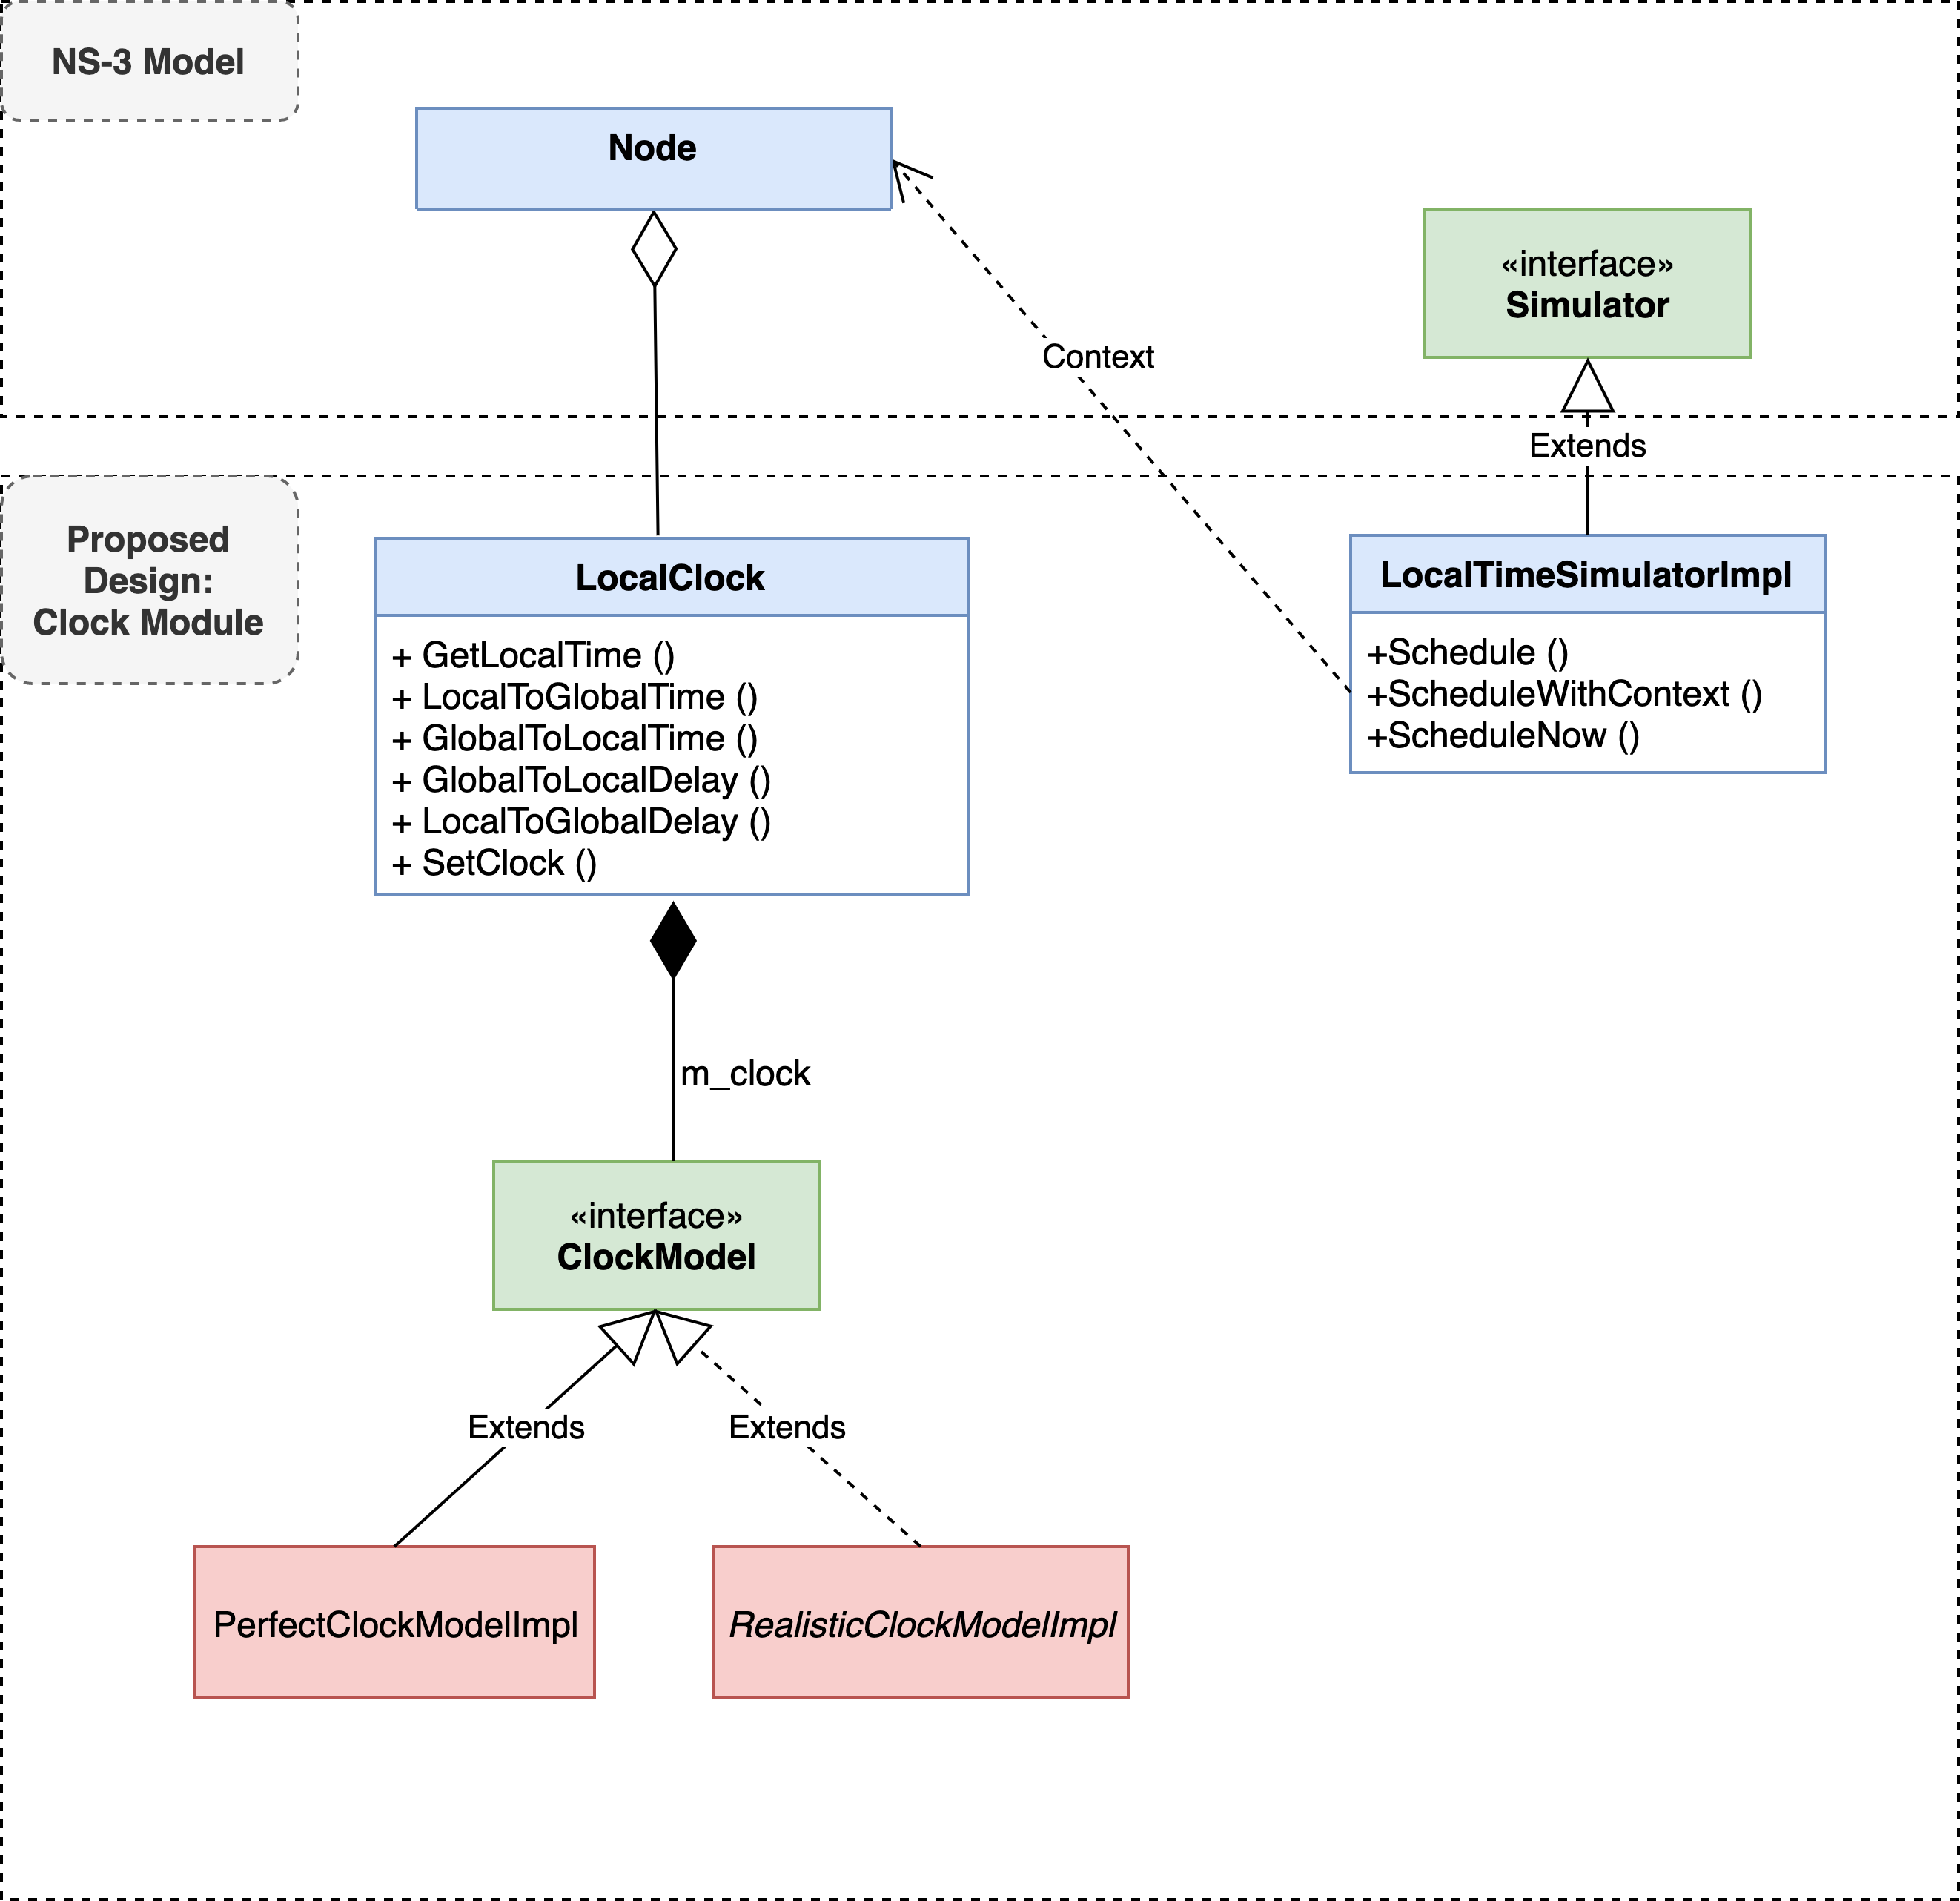
\includegraphics[width=.8\linewidth]{Figures/UMLSimulator.png}
\caption{UML design}
\label{fig:UMLDesign}
\end{figure*}

\subsubsection*{Clock Model}

\textit{ClockModel} is the interface for the clock behavioral model. It provides the minimum set of functions that a clock model should implement. 
Any clock model developed should extend from this interface. In order to introduce the notion of local time in ns-3, the clock model must provide a mapping between the local time and the simulator time (also called global time, or true time). The relative time-function can capture clock non-idealities in order to introduce realistic clocks. We are aware about the difficulty of creating realistic clock models as mentioned in \cite{ClockModelDiscussion}. However, the development of realistic clock models its out of the scope of this project. We present the interface that a clock model should use in order to be introduced in ns-3 and we provide a basic implementation: \textit{PerfectClockModelImpl}.
% #TODO
We believe that this paves the way towards achieving realistic simulations with realistic clock models. 

\subsubsection*{Local Clock}
A \textit{LocalClock} object is aggregated to every \textit{Node} using the ns-3 aggregation system. It represents the interface between the clock model and the node. 
It also tracks all the events that have been scheduled by this node with the purpose of rescheduling them if needed by an update of the clock model. Events are rescheduled when 
the \textit{ClockModel} for this \textit{Node} is updated using the \textit{SetClock()} function (to simulate an update of the clock's frequency for example). If some events have been scheduled using the previous clock model, then the mapping from local time to global time is no more valid for these events, so the \textit{LocalClock} class reschedule them in accordance to the newly provided clock model.

To do so, events are retrieved from the event list of the \textit{LocalClock} object and new execution times in the global time are calculated. New events are scheduled with the same \textit{EventImpl} (using a copy of the pointer).
Old events (which execution time does not correspond to the new clock) need to be removed from the scheduler. However, if events are cancelled using
\textit{Simulator::Cancel()}, it would be impossible to execute the event implementation provided to the new event. Indeed, in ns-3, \textit{Simulator::Cancel()} cancels the \textit{EventImpl}, not the \textit{EventId}. To avoid this problem, old events along with new events are pushed to the \textit{CancelEventsMap} map of \textit{LocalTimeSimulatorImpl}. 

The main attribute of the class \textit{LocalClock} is \(m\_clock\), which is a pointer of type \textit{ClockModelImpl} to the current clock model for this \textit{Node}. 

\subsubsection*{Simulator implementation}
The main differences between \textit{LocalTimeSimulatorImpl} and \textit{DefaultSimulatorImpl} are: 
\begin{itemize}
    \item  When an event is scheduled using the \textit{ Simulator::Schedule()} function, the delay is understood as being a local-time delay. The delay is then translated into a global-time delay before being inserted into the scheduler (the scheduler only operates in the global-time domain, and there is only one scheduler object, as in the current ns-3 code). See Figure \ref{fig:EventTimeTrans}.
    \item When a clock model is updated, \textit{LocalTimeSimulatorImpl} keeps track of the events that have been rescheduled, and will not execute the old events.
\end{itemize}

\begin{figure*}%[tbhp]
\centering
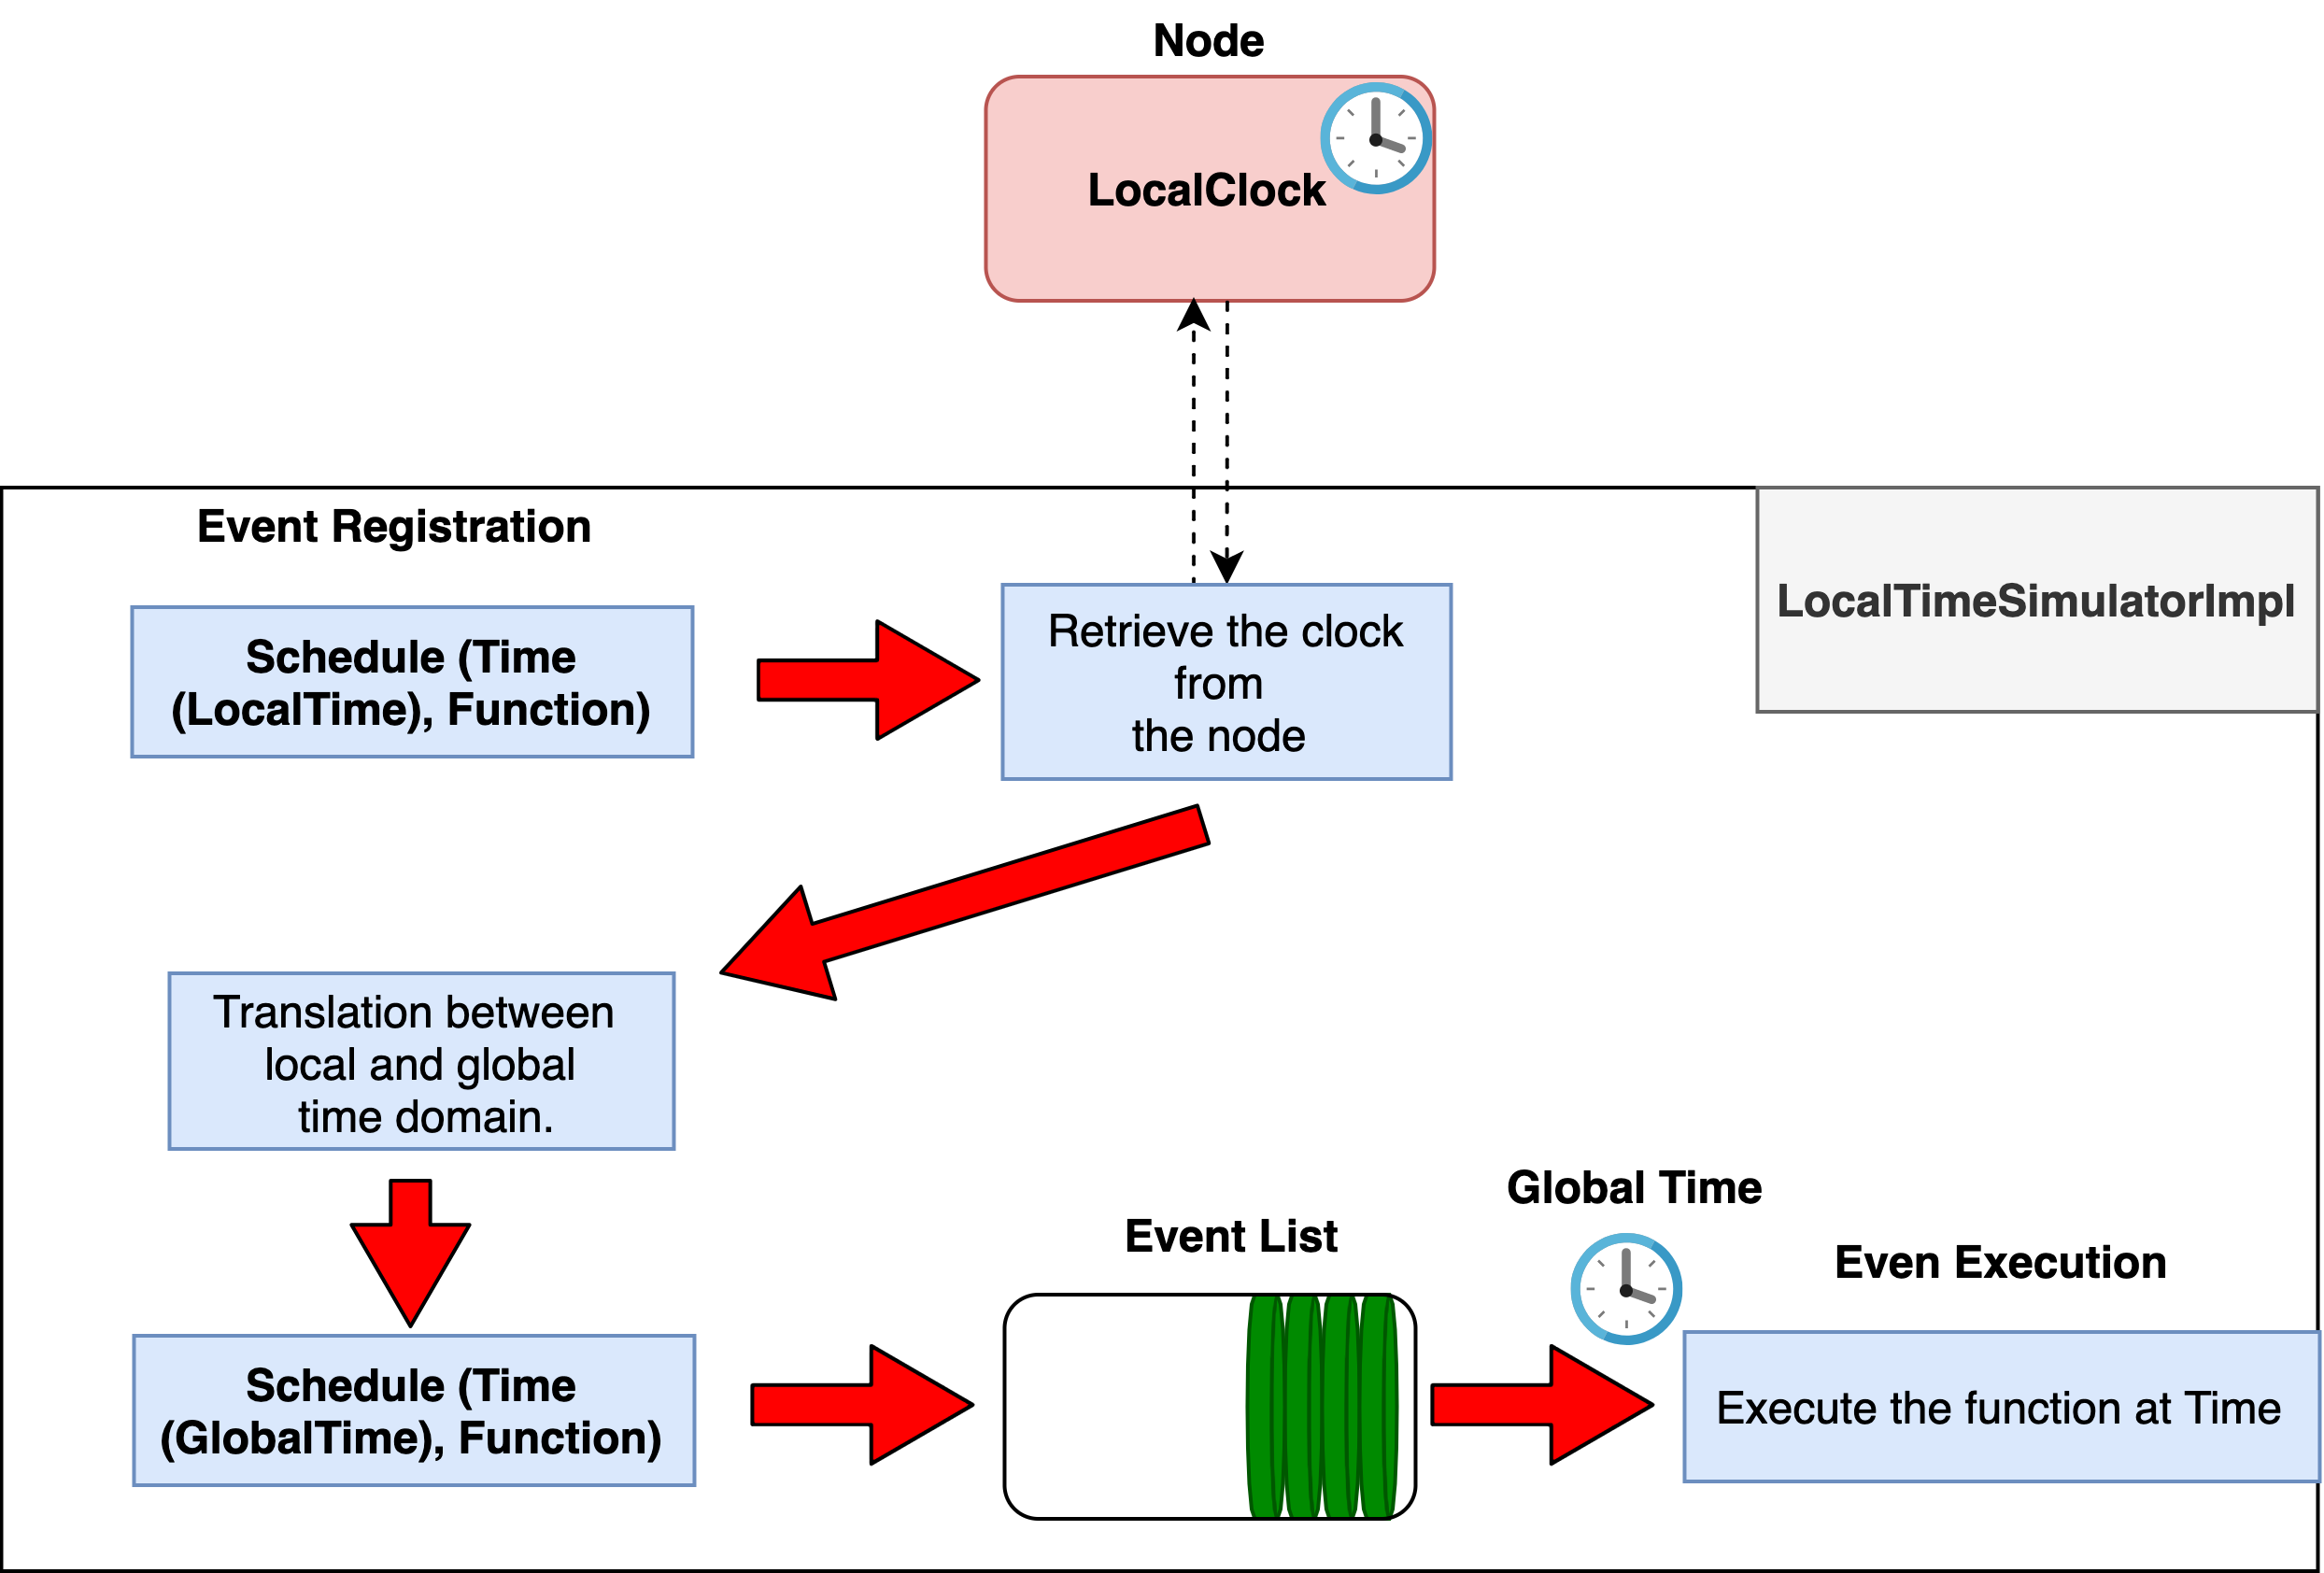
\includegraphics[width=.8\linewidth]{Figures/EventQueueTrans1.png}
\caption{Simulator steps for time translation when Schedule() is called}
\label{fig:EventTimeTrans}
\end{figure*}

When \textit{Simulator::Schedule()} is called, the \textit{Node} object is retrieved from the \textit{NodeList} using the current context of the simulator. When the context do not correspond to any node, delays are considered to be in global time.
%Context that do not correspond to any node are avoided in the simulator. 
% #TODO "avoided" ? what does it mean ?
Once the \textit{Node} object is retrieved, \textit{node->GetObject <LocalClock>()} is called to obtain the local clock, if aggregated\footnote{If the simulator doesn't find any aggregated \textit{LocalClock}, it assumes that this \textit{Node} relies on a perfect clock (local time = true time)}.
Using the \textit{LocalClock} object and its associated \textit{ClockModel}, the local-time delay is converted into a global-time delay. The event is inserted in the scheduler using the global-time delay. Last, \textit{LocalClock->InsertEvent()} is called in order to notify the \textit{LocalClock} that the event has been scheduled. The \textit{LocalClock} will keep track of it in case an update of the clock model requires to reschedule it.

When \textit{Simulator::ScheduleWithContext()} is called, the same actions as in \textit{DefaultSimulatorImpl} are taken. The delay is understood as being already a global-time delay. This is because:

$\bullet$ most of the \textit{ScheduleWithContext()} calls in today's ns-3 modules are related to a packet transmission within a channel. The delay is normally\footnote{The Point to Point device is the only device where the transmission delay is not decoupled from the propagation delay. This can be solve calling to the channel transmission function after TransmitComplete has elapsed.} the channel propagation time (e.g. with \textit{CsmaNetDevice}), which does not depend on the node clock. In particular, if a bit is `on the wire' when a clock update is triggered on the sending node, the global-time value at which the bit is expected to reach the remote end is not changed. So we typically don't need to keep track of these events and we don't reschedule them after a clock update.  
%TODO Maybe comment smth about p2p devices.

$\bullet$ the signature of \textit{ScheduleWithContext()} does not allow to retrieve any \textit{EventId}. Hence, even if we translate the time from local to global, we would never be able to reschedule or cancel the event. Is not recommended to change the signature of this function as discussed in \cite{ScheduleDiscuss}.

When \textit{Simulator::ScheduleNow()} is called, a call to the \textit{Schedule()} function with local-time delay 0 is done.

One of the things to take into account is that \textit{Simulator::Now()}  returns the current global time and not the local time. This is because most of the \textit{Simulator::Now()} calls in today's ns-3 are used to log or print the time at which an event occurs - and we definitively want the logs to be only prompted in the unique global-time domain. If the current local time is specifically required, it should be retrieved from the \textit{LocalClock->GetLocalTime()} function.
%TODO Adversarial cases where ::NOW() is called and LT should be return.

Another particularity of this implementation resides in the \textit{CancelEventsMap} map located in \textit{LocalTimeSimulatorImpl}. When events are rescheduled, old events id (as key) with their corresponding new events (as value) are inserted in this map. As explained in the \textit{LocalClock} section, we cannot use  \textit{Simulator::Cancel()} to remove old events or their implementation would be lost.
In order not to execute events that should not be invoked (because the execution time attach to the event does not correspond to the new clock of
the node), the \textit{ProcessOneEvent()} function is slightly modified and checks the CancelEventsMap. If the EventId that is going to be executed is found as a key in the map, the event is skipped.

Other problem arises from the fact that, after some rescheduling of events, the original \textit{EventId} is no more valid. Any process (i.e Applications) that schedule events will never realize about the change of the \textit{EventId} due to the rescheduling. Therefore, there is a need to map between the original events and the rescheduled events. Suppose the following situation of figure \ref{fig:IsExpired}. An event with id \(E_{1}\) is scheduled by an application at some point in the future. Because the local clock runs slower, the event is moved even further in the global time. At some point, a clock update is triggered, creating a new \textit{EventId} \(E^{'}_{1}\) adjusted to the new local clock. The application only has the reference to \(E_{1}\) and is completely unaware of \(E^{'}_{1}\). Thus, when the \textit{IsExpired(\(E_{1}\))} function is called by the application, the answer of the simulator should be based on the new event \(E^{'}_{1}\) as shown on figure \ref{fig:IsExpired}. In order to cope with the problem, the \textit{CancelEventsMap} is used to obtain \(E^{'}_{1}\) from \(E_{1}\), and \textit{IsExpired(\(E_{1}\))} returns  \textit{IsExpired(\(E^{'}_{1}\))}. Moreover, this is also useful when cancelling events. When the \textit{Cancel()} function is called, the first step is to verify if the \textit{EventId} is expired. The event is cancelled only if it is not expired. In such a manner, if the application wants to cancel event \(E_{1}\), the simulator will first check if \(E^{'}_{1}\) is expired. Assuming \(E^{'}_{1}\) is not expired, the simulator will cancel the event implementation of \(E_{1}\), which is the same than \(E^{'}_{1}\). So, neither \(E_{1}\) nor \(E^{'}_{1}\) will be executed. 

%%The map is also useful when the \textit{IsExpired()} function is called. The return value will depend whether the event has been rescheduled or not. This is, when an event is rescheduled, a new event is introduced in the scheduler. Assume that \textit{IsExpired()} is called with the old EventId and that the new event is scheduled farther in time, at some point you could call \textit{IsExpired(EventId oldEventId)} which would depend in the new event. Thus, we need a way to map between the old event and the new event. 

\begin{figure}[h]
\centering
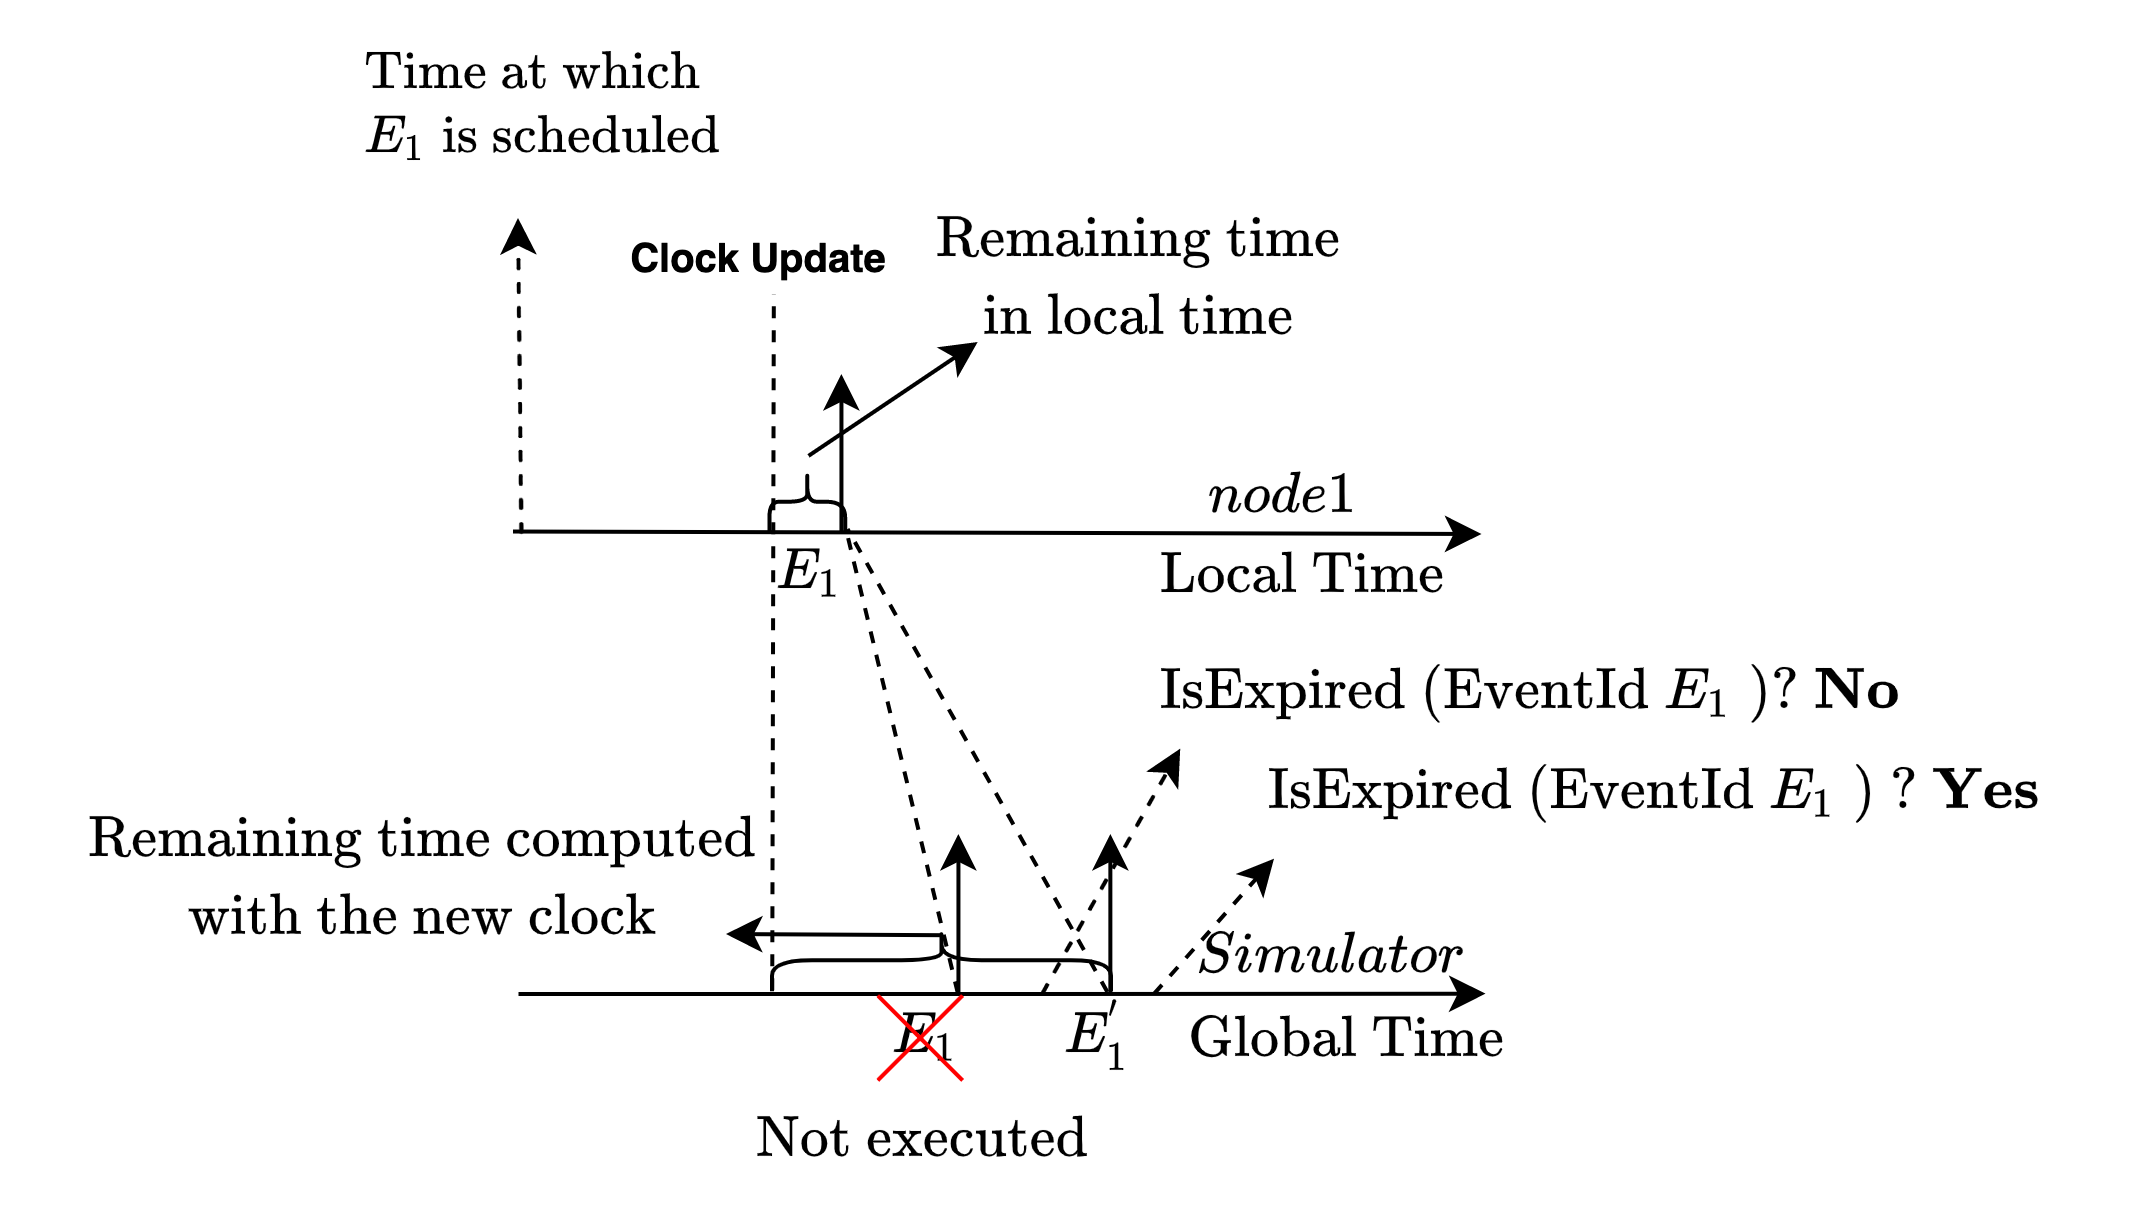
\includegraphics[width=\linewidth]{Figures/rescheduleExpired.png}
\caption{IsExpired () function when event rescheduling}
\label{fig:IsExpired}
\end{figure}

\section*{Validation}
The clock model validation have been done using both examples and test. Unitary tests have been written to verify the internals of \textit{LocalTimeSimulatorImpl} and \textit{LocalClock} classes using \textit{PerfectClockModelImpl}. They can be found in src/test/clock-test.cc.
Here we present the main characteristics of the two-clocks-simple.cc available in src/clock/example.

The scenario model is shown in figure \ref{fig:SimulationScenario} and the simulation parameters are in table \ref{tab:ScenarioParamsSimple}. 

\begin{figure}[h]
    \centering
    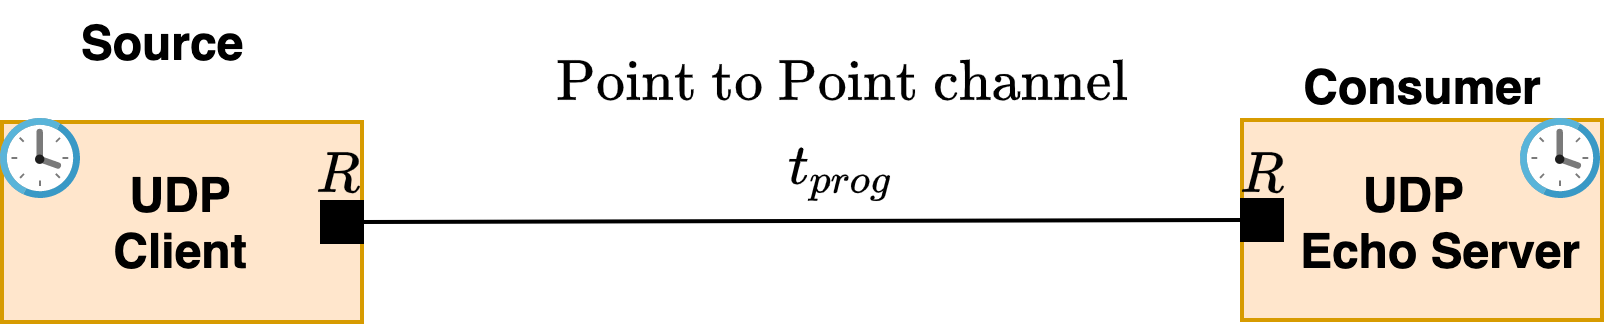
\includegraphics[width=0.8\linewidth]{Figures/ClockValidationScenario1.png}
    \caption{Simulation Scenario }
    \label{fig:SimulationScenario}
\end{figure}
\begin{table}[h]
    \centering
    \begin{tabular}{|p{3cm}|p{2.3cm}|p{2.3cm}|}
       \hline
         \textbf{Scenario Settings} & \textbf{Node 1} & \textbf{Node 2}  \\ [0.5ex] 
         \hline\hline
         Application & UDPClient & UDPEchoServer  \\ 
         \hline
         Interval Time (s) & 3 &\\
         \hline
         Net Device & Point to Point  & Point to Point  \\
         \hline
         Data Rate & 5mbps & 5mbps  \\
         \hline
         Packet Size (bytes) & 1024 & 1024 \\
         \hline
         Propagation Delay & 2ms & 2ms \\
         \hline
         Simulation (s) Time & 100 & 100 \\ 
         \hline
         Clock & Non-ideal & Ideal \\
         \hline 
    \end{tabular}
    \caption{Validation scenario parameters}
    \label{tab:ScenarioParamsSimple}
\end{table}

The scenario uses two nodes connected by point-to-point net devices. \textit{UdpClient} and \textit{UdpEchoServer} applications are installed on the nodes to generate the traffic. The client has a non-ideal clock using the \textit{PerfectClockModelImpl} class. This class allows to define the relative time-function between the global time and the local time. The relative time-function, shown in figure \ref{fig:NonIdealClock},is defined by a set of affine functions with a frequency offset (the slope of the function) as well as an initial offset (initial value when global time equals 0). When the fractional frequency offset is bigger than one, the local clock runs faster than the global time. On the other hand, when the fractional frequency offset is below one, the local clock runs slower. Likewise, when set to one, the clock runs at the same speed as the global time and is considered to be a perfect clock. 

In order to build the shape of the function, we use several \textit{PerfectClockModelImpl} objects and we trigger several clock updates to switch from one to the other: every 20 seconds, the clock update changes the frequency offset between clocks. In order to provide time continuity at each update, the initial offset of the function has to be re-computed. 
The relative time-function could also have been written as a single function, using a single clock model object, in which case we don't need the clock updates. 
Conversely, the server node runs a perfect clock. 

In order to make the \textit{clock} model run in the example, few changes need to be done in the main file. Remark, that the \textit{clock} module can run with the preexisting code of ns-3. A few changes need to be done while coding the scenario model in the main file. The changes are as follows:

$\bullet$ First, the global variable \textit{SimulatorImplementationType} needs to be changed, pointing to the \textit{LocalTimeSimulatorImpl}.
\begin{lstlisting}[language=C++]
    GlobalValue::Bind ("SimulatorImplementationType", StringValue ("ns3::LocalTimeSimulatorImpl"));
\end{lstlisting}
  
$\bullet$ Second, The \textit{ClockModel} implementation has to be created. In the case of the example, we use the \textit{PerfectClockModelImpl}.
\begin{lstlisting}[language=C++]
Ptr<PerfectClockModelImpl> clockImpl = CreateObject <PerfectClockModelImpl> ();

clockImpl -> SetAttribute ("Frequency", DoubleValue (freq));

clockImpl -> SetAttribute ("Offset", TimeValue (init_offset));

\end{lstlisting}
$\bullet$ Third, the \textit{LocalClock} object must be created,  the attribute m\_clock set, and the object aggregated to the node. 
\begin{lstlisting}[language=C++]
Ptr<LocalClock> clock = CreateObject<LocalClock> ();

clock -> SetAttribute ("ClockModelImpl", PointerValue (clockImpl));

node -> AggregateObject (clock);

\end{lstlisting}

The full code for the example can be found in /src/clock/examples/two-clocks-simple.cc 


\begin{figure}[h]
    \centering
    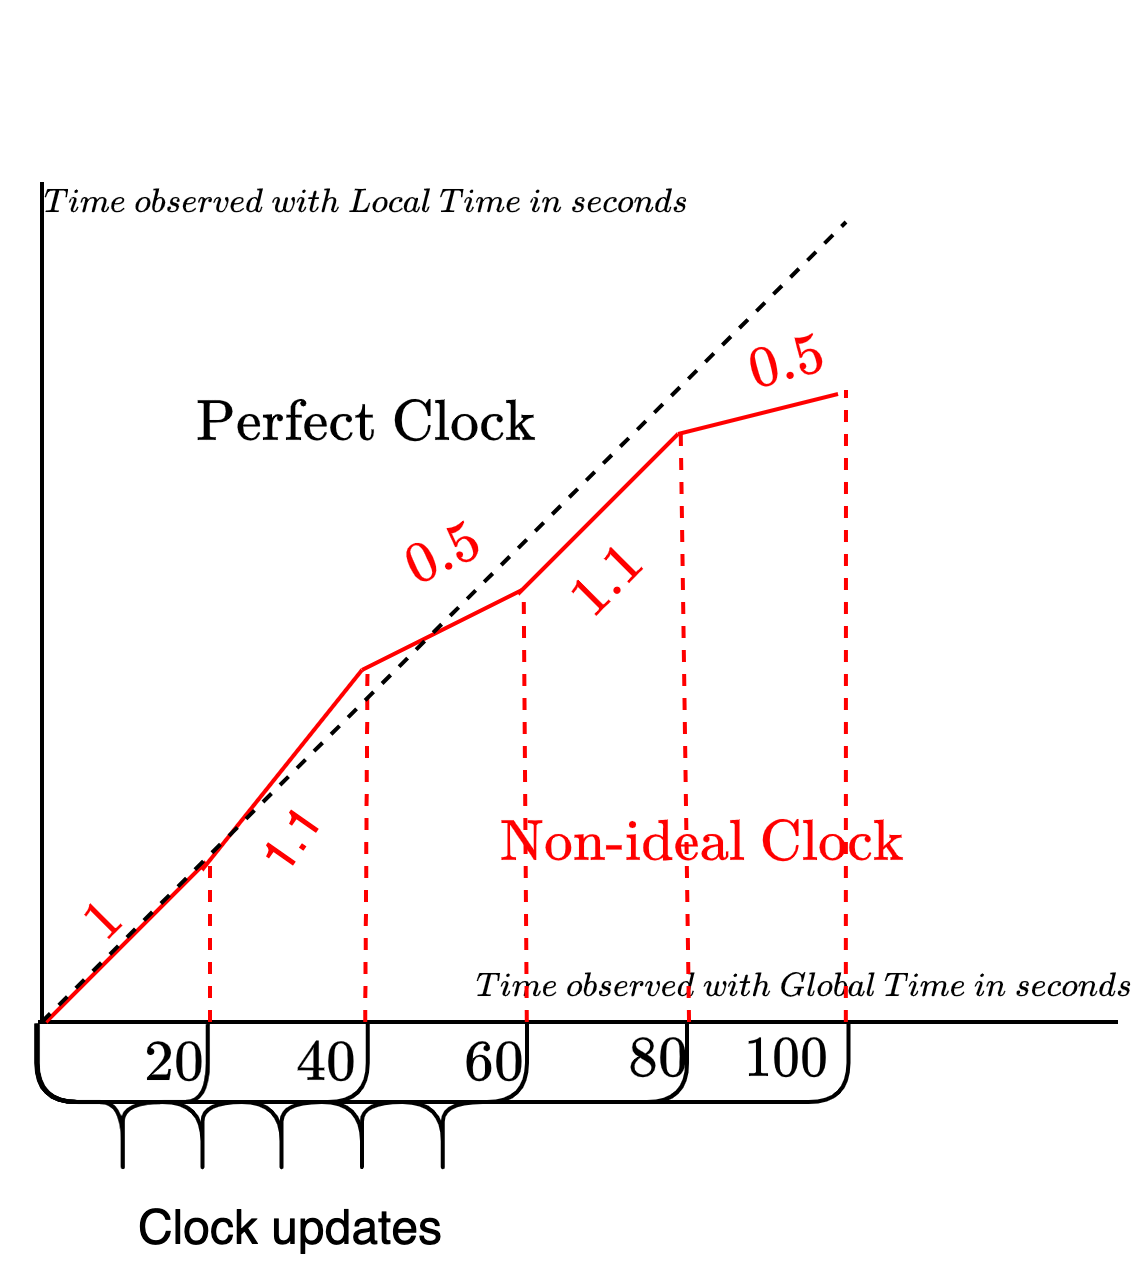
\includegraphics[width=0.8\linewidth]{Figures/ClockPatternValidation.png}
    \caption{Ideal and Non-Ideal clock model }
    \label{fig:NonIdealClock}
\end{figure}

Figure \ref{fig:ValidationGraph} shows the result obtained in the simulation. We represent the time at which the client node sends packets. As can be appreciated, the time at which packets are sent variates slightly depending on the frequency offset of the local clock. To compare the performance, we plot the same simulation, but without using the \textit{clock} module. We can see how the clock on the client tends to go slower.   

Between seconds 0 and 20, both clocks have same the frequency. However, after second 20 seconds, a clock update is triggered. This clock update modifies immediately the packets that are scheduled. As can be seen, straight after second 20 the slope increases, having the client clock running faster. The interval between packets change from 3 seconds to 2.7 seconds. Immediately after second 40 the slope decreases moving the interval time from 2.7 to 6 seconds. As we can see the frequency difference directly affects at which time packets are sent.

\begin{figure}[h]
    \centering
    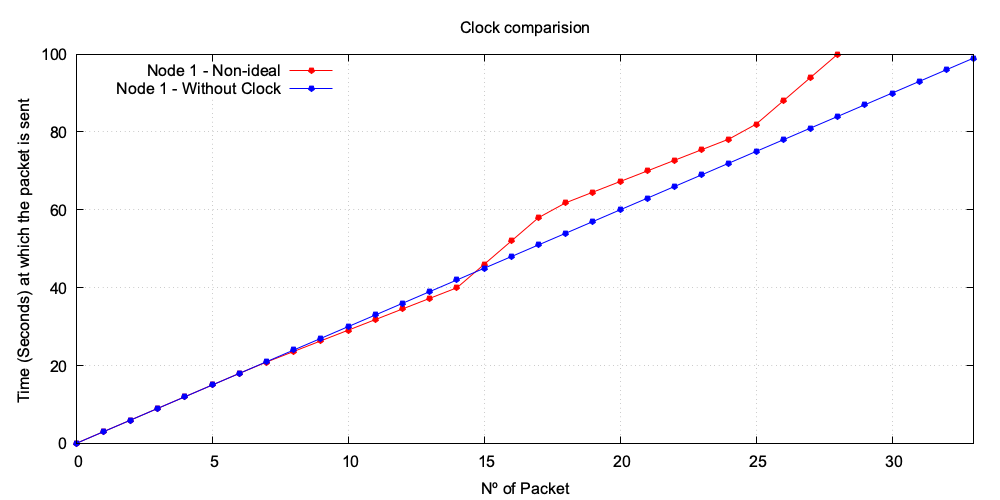
\includegraphics[width=\linewidth]{Figures/Validation2Nodes.png}
    \caption{Results obtained for Ideal and Non-Ideal clocks}
    \label{fig:ValidationGraph}
\end{figure}

\section*{Performance test}
For the purpose of evaluating the overhead added by the module, the computation time has been taken into account. A flexible scenario has been considered, where the parameters such as the number of nodes and the clock models can be tuned.  
Half of the nodes in the network communicate with the other half through a switch. The application generates random data flows within some intervals of time. Nodes can be tuned without clocks, with clocks and with clock updates. In such a way that the three possible scenarios are tested. Remark that clock updates affect all the nodes of the network. 
Simulation have been performed with 50 nodes  \ref{fig:50nodes}, 100 nodes \ref{fig:100nodes}, 200 nodes \ref{fig:200nodes} and 500 nodes \ref{fig:500nodes}.

The computer used for this testing uses an Intel Core i5 6200U Processor with 8GB RAM and Ubuntu 20.04. Ten simulations for each scenario have been carried out in order to have an average value of the computation time. In order to compute the values, \textit{Time} linux command has been used. 


\begin{figure}[h]
\centering
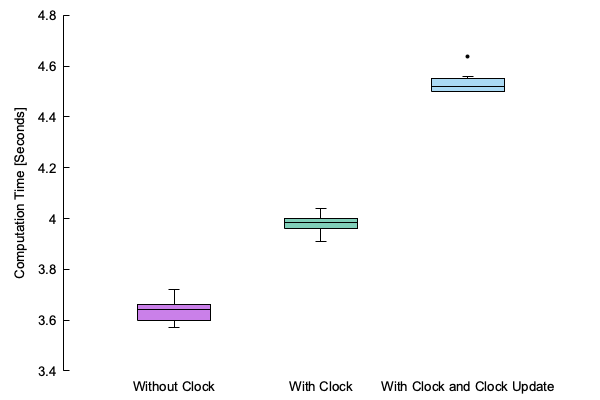
\includegraphics[width=.8\linewidth]{Figures/computation50.png}
\caption{Computation time with 50 nodes}
\label{fig:50nodes}
\end{figure}
\begin{figure}%[tbhp]
\centering
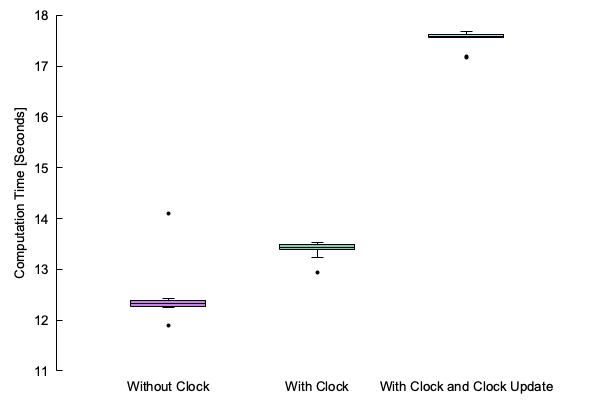
\includegraphics[width=.8\linewidth]{Figures/computation100.png}
\caption{Computation time with 100 nodes}
\label{fig:100nodes}
\end{figure}
\begin{figure}%[tbhp]
\centering
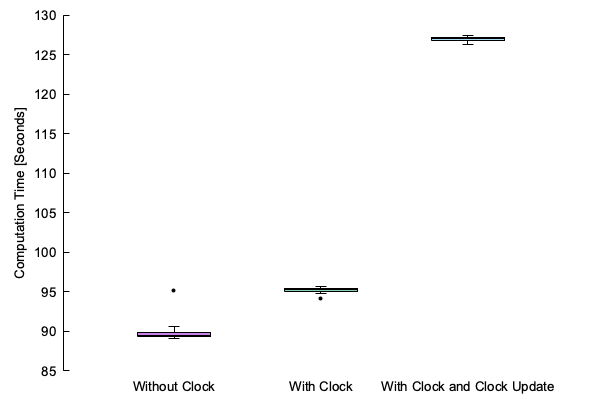
\includegraphics[width=.8\linewidth]{Figures/computation200.png}
\caption{Computation time with 200 nodes}
\label{fig:200nodes}
\end{figure}
\begin{figure}%[tbhp]
\centering
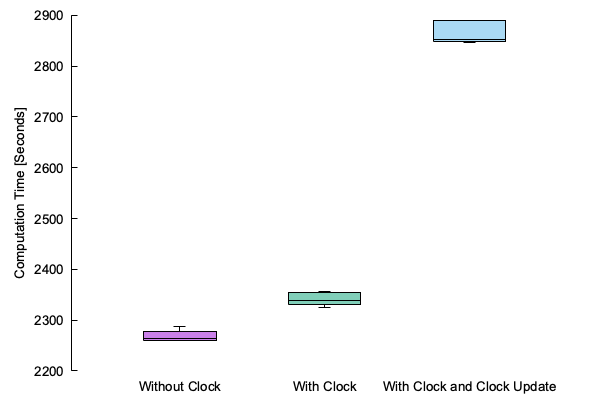
\includegraphics[width=.8\linewidth]{Figures/computation500.png}
\caption{Computation time with 500 nodes}
\label{fig:500nodes}
\end{figure}

As we could expect, the computation time increase with the number of nodes, as well as, with the different configurations of the clocks. Simulations show that in the case of using clocks, the increment in time is around a 3\% and 9\%, with respect to the simulation without clocks. However, when using frequent clock updates, the simulation time skyrockets from 3\% to 40\% for simulations with bigger number of nodes. As we can see, this increase in time can be a drawback with big and complex scenarios that require constant clock updating and more computing resources. 
\section*{Bibliography}
\bibliography{references}


\captionsetup*{format=largeformat}

\end{document}
